\section{Psicoacustica}

Altro aspetto da tenere in considerazione è il nostro sistema uditivo. In un sistema lineare in frequenza data in input una lista di frequenze, l’output conterrà le stesse, anche se magari dissimili in ampiezza e fase.
Il nostro apparato uditivo, infatti, a causa di secoli di evoluzione e cambiamenti ha sviluppato dei comportamenti che non lo rendono un sistema lineare, portando dunque a delle inesattezze dal punto di vista percettivo.
Ecco alcuni esempi di fenomeni di non linearità a cui siamo sottoposti:

\begin{itemize}
\item Distorsione armonica:
È la percezione di armoniche superiori di un tono puro. Questa distorsione può essere dovuta ad una pressione eccessiva dell’onda sul timpano;
\item Tono di combinazione:
Detto anche \textit{“terzo suono di Tartini”} è un effetto psicoacustico che comporta nella percezione di un terzo suono, nonostante in input i suoni siano stati solo 2.
La frequenza del tono ricostruito non sarebbe altro che la differenza tra i 2 toni di partenza
\item Curve isofoniche:
Il fenomeno delle curve isofoniche comporta una diversa percezione di ampiezza a per diverse frequenze ma aventi stesso SPL. Per fare un esempio una sinusoide da 1000 Hz a 110 Db SPL ha la stessa percezione di una sinusoide da 3000 Hz ma a 100 Db SPL (ballou - Handbook for Sound Engineers - 2008 - pag 43).
\end{itemize}

\begin{figure}[h]
\centering
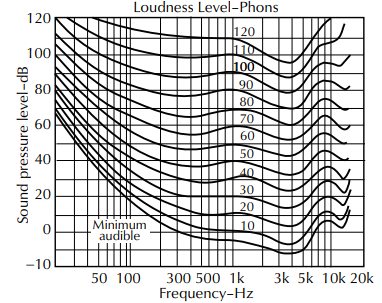
\includegraphics[width=0.80\textwidth]{isofoniche}
\caption{Grafico che mostra il comportamento delle curve isofoniche}
\label{fig:isofoniche}
\end{figure}

Questo è anche il motivo per il quale siamo più sensibili nella banda intorno ai 4 KHz, comportando dolore nell’ascoltatore se sottoposto a db elevati.

\subsection{Percezione della distanza}

Più interessante ai fini della tesi è la percezione della distanza, tema chiave nello studio degli spazi e della propagazione del suono.
È noto che, duplicata la distanza tra fonte sonora e ascoltatore, il SPL decade di 6 dB.
Nonostante questo, affinché abbiamo la percezione della duplicazione della distanza c’è bisogno della diminuzione di almeno 20 dB (j. Blauert spatial hearing).

Un elemento che però ci permette di comprendere quando una fonte è lontana è la sua composizione spettrale, infatti, a causa dell’assorbimento dell’aria (del mezzo per essere più precisi) le frequenze alte saranno assorbite maggiormente, comportando una presenza più elevata di basse frequenze.

Per questo, in modo tale da replicare distanza e vicinanza dalla fonte sonora, oltre a questi accorgimenti è da tenere in considerazione il rapporto tra suono diretto e riverberato.
In un ambiente reale infatti, è proprio il rapporto tra le due sorgenti a determinare dove e quanto è distante un evento sonoro.
